\section{Design}
\label{sec:design}
\fxfatal{Design}

This chapter presents the implemented framework \textit{Banshie} (Benchmark Framework for Information Extraction). The requirements, architecture, design and concrete implementation details are explained and discussed on the following pages.

\subsection{Analysis and requirements}
Provide a platform to benchmark domain-specific information extraction modules.

Designed for Extension and Modularity
OSGi-aware
State of the Art patterns: DI, IoC, Composition over Inheritence, ...
Open Source (Github!)

\url{https://github.com/whiskeysierra/banshie}

\subsection{Architecture}
OSGi, module hierarchy, dependencies

\newpage
\begin{figure}[H]
\centering
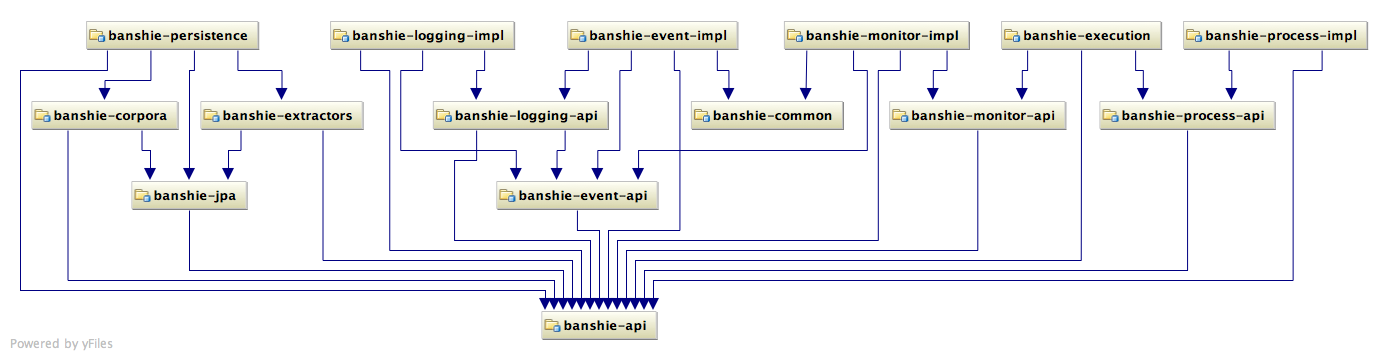
\includegraphics[angle=90, width=0.42\textwidth]{module-dependencies.png}
\caption{Module dependencies}
\label{fig:module-dependencies}
\end{figure}

\newpage
\subsection{Technologies}

\subsubsection{Dependency Injection}
\gls{DI} is an expression introduced by Martin Fowler in its article \textit{Inversion of Control Containers and the Dependency Injection Pattern} \cite{Fowler:2004}. Dependency Injection specifies the means for obtaining objects in such a way as to maximize reusability, testability and maintainability compared to traditional approaches such as constructors, factories, and service locators \cite{JSR330}. \gls{DI} does this by allowing a class to specify its dependencies and rely on their provision at runtime rather than retrieving them explicitly. This leaves the programmer's code clean, flexible, and relatively free of dependency-related infrastructure \cite{JSR330}.

\paragraph{Guice}
Guice is a lightweight dependency injection framework for Java \cite{Guice}. It's open source and available on \url{https://code.google.com/p/google-guice/}.

The typical code to implement is shown in the following two listings. The first shows a simple \textit{Module}. Modules in Guice are usually used to bind interfaces to concrete classes.

\begin{listing}[H]
\begin{minted}{java}
public final class ProcessModule extends AbstractModule {

    @Override 
    protected void configure() {
        bind(ProcessService.class).to(DefaultProcessService.class);
    }

}
\end{minted}
\caption{Guice module}
\end{listing}

In your classes you usually define a single constructor, annotated with \texttt{@Inject}, and all required dependencies as parameters. The construction of instances and the dependency resolution is done by Guice, no additional boilerplate code is necessary.

\begin{listing}[H]
\begin{minted}{java}
final class DefaultEngine implements Engine {

    private final ProcessService service;

    @Inject
    DefaultEngine(ProcessService service) {
        this.service = service;
    }

}
\end{minted}
\caption{Constructor injection}
\end{listing}

\paragraph{Guice Extensions}
Guice has an extensible plug-in mechanism which allows third parties to provide additional functionality. Banshie uses two official Guice extension extensively: Assisted Inject\footnote{\url{https://code.google.com/p/google-guice/wiki/AssistedInject}} and Multibindings\footnote{\url{https://code.google.com/p/google-guice/wiki/Multibinding}}. Assisted Inject allows the combination of Guice-provided dependencies and user-provided parameters on a single injection point. Multibindings supports the binding and injection of Sets and Maps.

\paragraph{Peaberry}
Guice has no native OSGi support, apart from maybe the OSGi-compatible bundle manifest. To overcome this shortcoming, Peaberry\footnote{\url{https://code.google.com/p/peaberry/}}, a third-party open-source Guice extension offers OSGi-Guice bridge capabilities. It offers \gls{DI} of OSGi dynamic services via Guice's common injection mechanisms and provides a rich an typesafe API to deal with the OSGi service registry and service lifecycle events. Peaberry even supports the automatic \gls{DI} context creation upon bundle start by using an OSGi extender bundle. Bundles just need to provide the following bundle header to trigger an execution:

\begin{listing}[H]
\texttt{Bundle-Module: org.whiskeysierra.banshie.execution.ExecutionModule}
\caption{Peaberry bundle header}
\end{listing}

\subsubsection{Persistence}

\paragraph{OpenJPA}

\paragraph{Aries}

\paragraph{Derby}

\paragraph{Jackson}

\subsubsection{Build tools and source code management}

\paragraph{Ant and Maven}

\paragraph{Bundle Plugin}
BND Tool

\newpage
\subsection{API}

\begin{figure}[H]
\centering
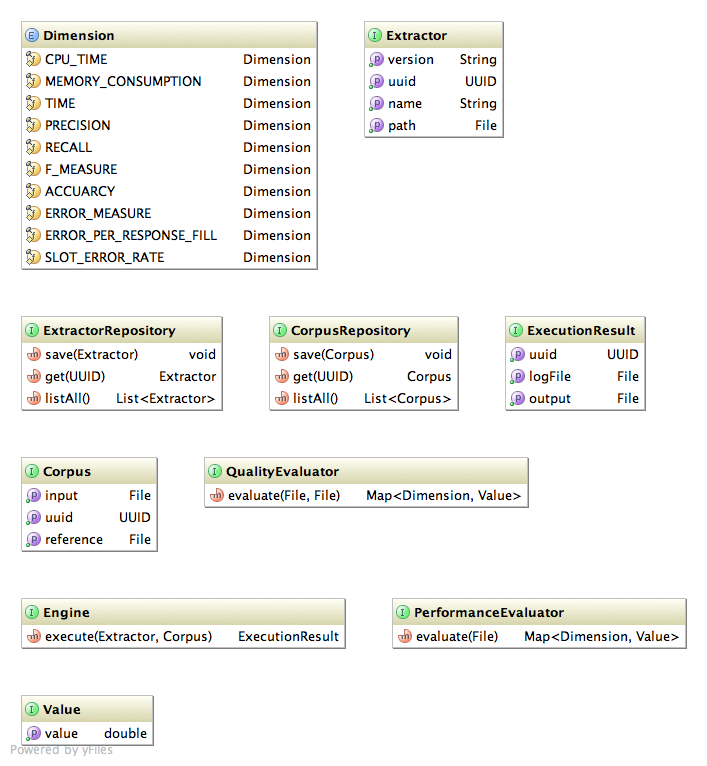
\includegraphics[width=0.9\textwidth]{api.png}
\caption{Banshie API diagram}
\label{fig:api}
\end{figure}

\newpage
Listing \ref{lst:usage} shows the simple basic steps required to perform a single extractor evaluation evaluation.

\begin{listing}[H]
\begin{minted}{java}
// via dependency injection or direct instantiation
final ExtractorRepository extractors = ...;
final CorpusRepository corpora = ...;
final Engine engine = ...;
final PerformanceEvaluator performance = ...;
final QualityEvaluator quality = ...;

final Extractor extractor = extractors.get(extractorId);
final Corpus corpus = corpora.get(corpusId);

final ExecutionResult result = engine.execute(extractor, corpus);
final Map<Dimension, Value> p = 
    performance.evaluate(result.getLogFile());
final Map<Dimension, Value> q = 
    quality.evaluate(corpus.getReference(), result.getOutput());

// handle evaluation results
...
\end{minted}
\caption{Banshie API usage}
\label{lst:usage}
\end{listing}

\subsection{Extractor interface specification}
Java 6+, executable Jar file (jarjar, resources, ...), Manifest, MainClass header, plain text document stdtin, xml stdout

\begin{listing}[H]
\inputminted{xml}{../../../../../banshie-api/src/main/resources/schema.xsd}
\caption{Banshie XML Schema}
\label{lst:xml-schema}
\end{listing}

\begin{listing}[H]
\inputminted{xml}{../../../../../banshie-api/src/main/resources/example.xml}
\caption{Banshie XML Example}
\label{lst:xml-example}
\end{listing}